\documentclass[fontsize=12pt, a4paper]{scrartcl}
%\let\stdsection\section 	% neue seite für neues kapitel
%\renewcommand\section{\newpage\stdsection} 

% ### variables

\def \var_single_plot_width {0.49}
\def \var_double_plot_width {0.49}

% ### literaturverzeichnis
%\usepackage[sorting=none]{biblatex}
%\addbibresource{sim_axelsson.bib}

% ### sprachpakete
\usepackage[ngerman]{babel} % Deutsche Sprachanpassungen
\usepackage[T1]{fontenc}    % Silbentrennung bei Sonderzeichen
\usepackage[utf8]{inputenc} % Direkte Angabe von Umlauten im Dokument.
\usepackage{cite}

% ### grafiken   
\usepackage{graphicx}		% Zur Darstellung von Bildern
\usepackage{subcaption}
\usepackage{float}			% platziert figures am gewünschten platz
\usepackage[export]{adjustbox}% http://ctan.org/pkg/adjustbox
\usepackage{svg}
\usepackage{amsmath}
\usepackage{bm}

% ### matplotlib plots
\usepackage{pgf}
\usepackage{lmodern}% http://ctan.org/pkg/lm
%\usepackage{tikz}
\usepackage{pgfplots}
\pgfplotsset{width=10cm,compat=1.9}
%\pgfplotsset{compat=newest}

\usepackage{csquotes}

\usepackage[parfill]{parskip}

% ### curcuits
\usepackage{tikz}
\usetikzlibrary{arrows}
\usepackage[RPvoltages]{circuitikz}

% ### titleseite
\usepackage{titling}
\title{System-Modellierung einer Membranpumpe für die Mikro-Fluidik}
\author{Kristjan Axelsson, Timo Stubler}
\date{\today}               

% ### fancy features
\usepackage{hyperref}

\begin{document}
\setlength{\tabcolsep}{12pt} % set col spacing for tables
\pagenumbering{gobble}		% turn off page numbers
\begin{titlingpage}
\begin{center}
\begin{figure}[H]
    \centering
    \begin{subfigure}[B]{0.30\textwidth}
        
\includegraphics[width=\textwidth, valign=t]{bilder/Logo_MNM_EN_Farbe_ohneHM (1).png}
    \end{subfigure}
    \begin{subfigure}[B]{0.60\textwidth}
        
\includegraphics[width=\textwidth, valign=t]{bilder/Hochschule_Muenchen_Logo.png}
    \end{subfigure}
\end{figure}
\setcounter{figure}{0}
\vspace{2cm}
\begin{large} 
\textbf{\thetitle} \\
\end{large}
\vspace{1cm}
\theauthor\\
\vspace{1cm}
Hochschule München \\
Fakultät für angewandte Wissenschaften und Mechatronik \\
\vspace{1cm}
\thedate
\end{center}
\end{titlingpage}

\tableofcontents            % Inhaltsverzeichnis anlegen

% quelle \cite{pedrotti} \\
% siehe Abb. \ref{fig_detector_test} \\
% siehe Kap. \ref{fazit}

\newpage

\section{Einleitung}
\pagenumbering{arabic}		% turn on page numbers
Im Rahmen dieser Simulationsstudie wird eine piezoelektrische Mikromembranpumpe modelliert und optimiert. Die Pumpe wird durch ein fluidisches Ersatzmodel beschrieben welches analog zu einem elektrischen Ersatzmodel ist. Im theoretischen Teil dieser Arbeit werden die einzelnen Komponenten der Pumpe vorgestellt. Diese sind die Pumpkammer, zwei passive Klappenventile sowie die Zuleitungen und Reservoirs aus bzw. in welche ein Fluid gepumpt wird. Nachdem der Aufbau behandelt wurde werden die beiden Simulationsmodelle vorgestellt. Zuerst das Einzelstrang-Modell mit welchem die Ventile im Detail untersucht werden, gefolgt von einem Modell des Gesamtsystems das die Membranpumpe beschreibt. Mit diesem werden weitere charakteristische Eigenschaften des Systems untersucht. Die im Rahmen dieser Studie durchgeführten Simulationen umfassen die Simulation der Zuleitungen, die Untersuchung der Ventile auf Leckströme, die Leistung der Pumpkammer gegen erhöhte Reservoirdrücke zu arbeiten und abschließend die Bestimmung der Grenzfrequenz der Pumpe. Den Abschluss dieser Arbeit bildet eine kurze Zusammenfassung der Ergebnisse sowie ein Ausblick bzw. eine Vorarbeit für künftige Simulationsstudien im Rahmen der besuchten Vorlesung. Der Python-Code der Simulation ist im Anhang zu finden.

\section{Theorie}

Im Folgenden wird die Modellierung der Membranpumpe besprochen. Der Antrieb der Pumpe wird durch einen Piezoaktor realisiert. Dieser wird über eine Wechselspannung betrieben und erzeugt so abwechselnd einen Über- bzw. Unterdruck in der Pumpkammer. Die Ventile sind passive Klappenventile welche nur in eine Richtung öffnen. Je nach Anordnung dient dieses Ventil einmal als Auslass und einmal als Einlass. Die Klappenventile sind über einen Schlauch jeweils mit einem Reservoir verbunden.

Im Folgenden werden zwei Modelle vorgestellt. Das erste Besteht aus der Pumpkammer mit einem Klappenventil und einer Zuleitung welche an einem Reservoir angeschlossen ist (Einzelstrang). Dieses Modell dient der Untersuchung der Ventile auf Leckströme. Das zweite Modell umfasst die gesamte Pumpe welche auf ihre Funktionsweise bezogen auf Gegendruck, Antriebsfrequenz und Leitungsgeometrie untersucht wird (Gesamtsystem).

Für die Simulation wird ein fluidisches Ersatzmodell verwendet \cite{script}

\[ Widerstand \:\widehat{=}\:  Strömungswiderstand = \biggl[\frac{m^3/s}{Pa}\biggr] \]
\[ Kapazität  \:\widehat{=}\:  fluidische Kapazität = \biggl[\frac{m^3}{Pa}\biggr] \]
\[ Spannung  \:\widehat{=}\:  Druck = [Pa] \]

Dies führt für den Druckabfall über den Komponenten zu folgenden Beziehungen zwischen Druck \(P\), Fluidstrom \(\dot{V}\) und Strömungswiderstand \(R\).

\[Widerstand \rightarrow P = R\dot{V} \]
\[Kapazität \rightarrow P = \frac{V}{C} \]
\[Quelle \rightarrow P = P \]

\subsection{Leitungsströmung}
\label{subsec:reservoirsection}
Das Reservoir wird als unendlich groß angenommen und daher mit einem Konstanten Druck modelliert.


\[ P_r = Umgebungsdruck \]

Die Zuleitung wird durch einen einfachen Strömungswiderstand modelliert. Da für dieses Modell die Strömung als laminar betrachtet wird ist der Strömungswiderstand über das Gesetz von Hagen-Poiseuille zu beschreiben \cite{fluidmechanics}. Dabei ist \( r \) der Radius der Zuleitung, \(l\) die Länge, \(dP\) der Druck über dem Rohrabschnitt und \(\eta\) die Viskosität des Mediums.

\begin{equation}
	\dot{V} = \frac{\pi \cdot r^4 \cdot dP}{8 \cdot \eta \cdot l}
	\label{eq:hagenpois}
\end{equation}

Mit dem oben definierten Zusammenhang zwischen Fluidstrom \(\dot{V}\) und dem Druckabfall \(dP\) folgt für den Strömungswiderstand \(R\)

\begin{equation}
	R = \frac{8 \cdot \eta \cdot l}{\pi \cdot r^4}
\label{eq:leckagestrom}
\end{equation}

Ob die Einordnung der Strömung in den laminaren Bereich Gültigkeit behält wird anhand einer einfach Abschätzung für die Reynoldszahl geprüft. Für die Reynoldszahl in Rohrströmungen gilt folgender Zusammenhang:
 
\begin{equation}
	Re = \frac{v_{m} \cdot d}{\nu}
	\label{eq:reynoldstube}
\end{equation}

Die mittlere Geschwindigkeit kann mit dem Gesetz von Hagen-Poiseuille (Gleichung \ref{eq:hagenpois}) berechnet werden:

\begin{equation}
	v_m = \frac{\dot{V}}{A} = \frac{\pi \cdot r^4 \cdot dP}{8 \cdot \eta \cdot l \cdot A}
	\label{eq:meanvelocity}
\end{equation}

Um die maximale Reynoldszahl zu errechnen werden die Parameter eingesetzt, welche zur höchstmöglichen mittleren Geschwindigkeit der Leitungsströmung führen. Mit einem Leitungsradius von $r=0.5 mm$ ($A=0.79mm^2$) und einer Länge von $l = 100 mm$, maximaler Druckdifferenz zwischen Pumpkammer und Reservoir von $dP_{max} = 50 \cdot 10^{3} Pa$ sowie der dynamischen Viskosität von Wasser $\eta=1.002 \cdot 10^{-3} kg m^{-1} s^{-1}$ erhält man:

\begin{equation}
	Re = 1941.5 < 2040 = Re_{krit}
	\label{eq:Reynoldresult}
\end{equation}

Damit befindet man sich unterhalb der kritischen Reynoldszahl und damit im laminaren Bereich. In dieser Arbeit wird als Arbeitsfluid immer Wasser angenommen.

\subsection{Klappenventile}
\label{subsec:ventilsection}

Die Klappenventile werden durch Widerstandswerte beschrieben welche vom Druck abhängen. Für das vorwärts gerichtete Ventil (Auslass) gilt: Bei Drücken > 0 ist das Ventil geöffnet. Für Drücke < 0 ist das Ventil geschlossen. Für das nach hinten gerichtete Ventil (Einlass) gilt das Gegenteil. Die Widerstände für den geöffneten und geschlossenen Zustand werden über das oben beschriebene Gesetz von Hagen-Poiseuille abgeschätzt. Die Kennlinien der beiden Ventiltypen sind in Abbildung \ref{fig:ventilkennlinie} aufgezeigt.

\begin{figure}[H]
	\centering
	\begin{subfigure}[H]{0.48\textwidth}
		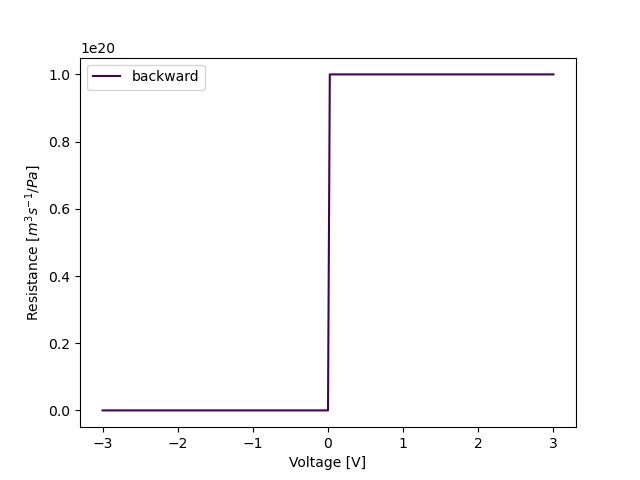
\includegraphics[width=\textwidth, valign=t]{bilder/Kennlinien/velve_backwards.png}
	\end{subfigure}
	\begin{subfigure}[H]{0.48\textwidth}
		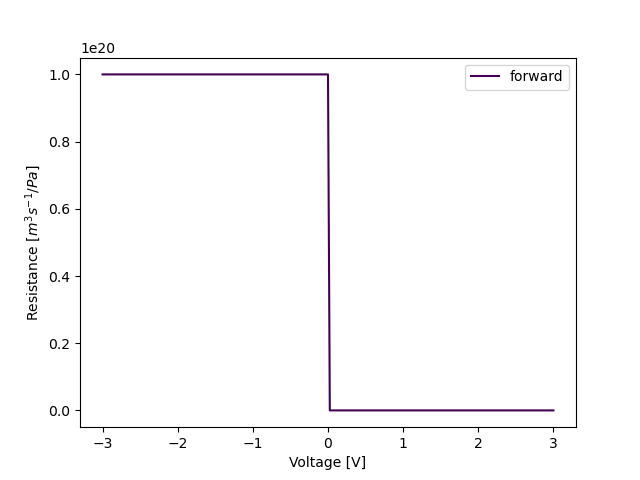
\includegraphics[width=\textwidth, valign=t]{bilder/Kennlinien/velve_forwards.png}
	\end{subfigure}
	\caption{Signalabhängiger Widerstandswert eines Klappenventils für den a) Einlass und b) Auslass}
	\label{fig:ventilkennlinie}
\end{figure}

\subsection{Pumpkammer}
Real wird die Auslenkung der Pumpkammer durch Anlegen eines elektrischen Signales erzeugt. Dadurch verändert sich der Druck in der Pumpkammer, sowie deren Kapazität. Die Pumpkammer ist in erster Näherung durch einen Kolben zu beschreiben (siehe Abbildung \ref{fig:kammerkonzept}). Die Höhe der Druckamplitude wird durch einen Proportionalitätsfaktor von der Spannung abhängig gemacht, ebenso die fluidische Kapazität. Die Extremwerte für Druck und Kapazität der Pumpkammer beruhen auf Erfahrungswerten \cite{internal}. Die Trägheit der Pumpkammer wird über ein RC Glied (PT-1) in erster Näherung berücksichtigt und wird mit einer abgeschätzten Zeitkonstante konkretisiert. Aus diesen Überlegungen ergeben sich für die Pumpkammer das in Abbildung \ref{fig:kammerkennlinie} dargestellte Verhalten für die Größen Auslenkung (Stroke), Kapazität und Druck, welche die Kennlinien darstellen.

\begin{figure}[H]
	\centering
	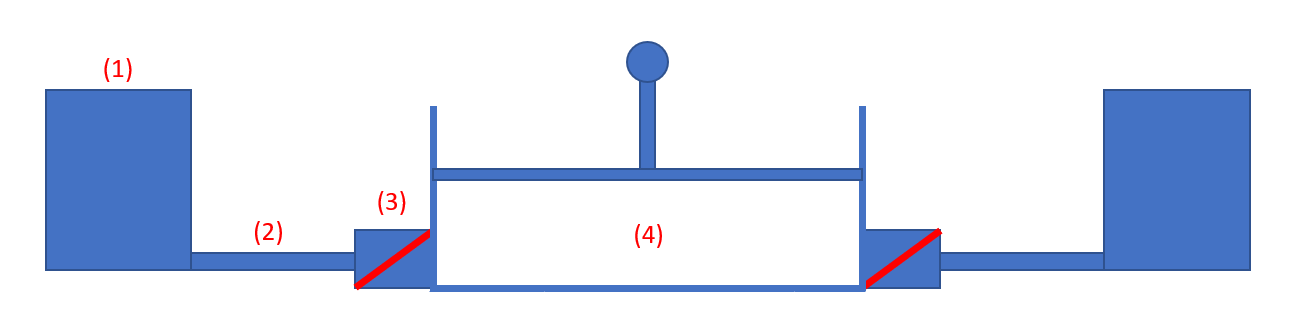
\includegraphics[width=0.98\textwidth]{bilder/theorie/pumpe_prinzipskizze.PNG}
	\caption{1) Reservoir 2) Zulauf 3) Ventil 4) Pumpkammer}
	\label{fig:kammerkonzept}
\end{figure}

\begin{figure}[H]
	\centering
	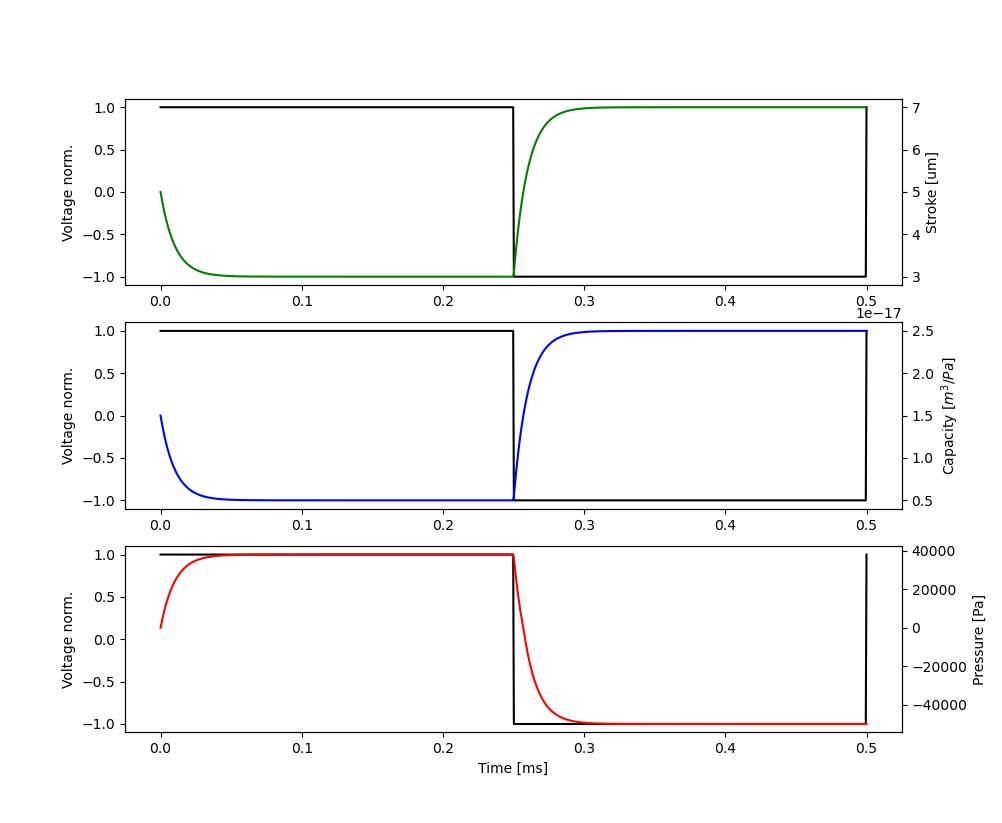
\includegraphics[width=0.98\textwidth]{bilder/Kennlinien/Chamber_kennlinie.PNG}
	\caption{Kennlinien der Pumpkammer für a) Druck-/Saughub b) Kapazität c) Druck}
	\label{fig:kammerkennlinie}
\end{figure}

\section{Modellierung}

Im Folgenden wird die Modellierung des Einzelstrangs und des Gesamtsystems behandelt. Wie bereits erwähnt, werden elektrische Ersatzschaltbilder herangezogen, welche dann mithilfe der elektrisch-fluidischen Analogiegesetze untersucht werden. Für die Simulationen wird von folgenden Basis-Parametern ausgegangen (siehe Tabelle \ref{tab:modelparameters}), welche aber in den Parameterstudien teilweise unter Variation stehen.

\begin{table}[H]
\begin{tabular}[h]{c|c|c|c|c|c|c}
	  & Wert & Einheit & & & Wert & Einheit\\
	\hline
	Leit. Längen & 100 & [mm] & & Sig. Amplitude & 1 & [-] \\
	Leit. Radien & 0.5 & [mm] & & Sig. Frequenz & 2 & [kHz] \\
	Ven. $R_{open}$ & 2e6 & [$\frac{m^3/s}{Pa}$] & & Sig. Offset & 0 & [-] \\
	Ven. $R_{close}$ & 1e20 & [$\frac{m^3/s}{Pa}$] & & PT-1, K & 1 & [-] \\
	Ka. $P_{min}$ & -38e3 & [Pa] & & PT-1, T & 1e-3 & [s] \\
	Ka. $P_{max}$ & 50e3 & [Pa] & & Sim. Time & 1e-3 & [s] \\
	Ka. $C_{min}$ & 0.5e-17 & [$m^3/Pa$] & & Sim. Steps & 1000 & [-] \\
	Ka. $C_{max}$ & 1.5e-17 & [$m^3/Pa$] & & Fluid Temp. & 293.15 & [K]
\end{tabular}
\caption{\label{tab:modelparameters} Model Parameters (Leit. = Leitungen, Ven. = Ventil, Ka. = Kammer, Sig. = Signal, Sim. = Simulation)}
\end{table}

\newpage

\subsection{Einzelstrang}

Das Gesamtsystem Pumpe kann in zwei Einzelstränge (ein-, ausleitend) unterteilt werden, welche jeweils einen in sich geschlossenen Kreislauf im Ersatzschaltbild darstellen.
Die Betrachtung eines Strangs kann analog auf den anderen übertragen werden. Folglich wird hier nur ein Strang erläutert.

\begin{figure}[H]
	\includesvg[scale = 0.6]{bilder/circuits/single_branch}
	\caption{Einzelstrang des Pumpensystems als elektrisches Ersatzschaltbild}
	\label{singlebranch}
\end{figure}

Der Eingangsdruck ($U_{in}$), der Reservoir-bedingt anliegt, bildet mit dem durch den Piezoaktor erzeugten Kammerdruck ($U_{Signal}(t)$) eine Druckdifferenz. Nach Hagen-Poiseuille resultiert daraus ein Volumenstrom in eine vom Vorzeichen der Druckdifferenz ($U_{Signal}(t)-U_{in}$) vorgegebene Richtung. Der Leitungswiderstand ($R_{T}$) und der Ventilwiderstand ($R_{V}$) begrenzen die resultierenden Volumenströme. Dabei beherbergt [wohnt der da!?!? :D] das Modell des Ventils eine Abhängigkeit von der Druckdifferenz. Im gezeigten Einzelstrang ist der Ventilwiderstand für negative Druckdifferenzen gering, für positive Druckdifferenzen sehr hoch, sodass das Ventil in diese Richtung schließt. Am Ende des Einzelstranges befindet sich die Pumpkammer und die Quelle des Drucksignals. Das Aufnahmevermögen der Pumpkammer wird durch ein Kondensatorelement beschrieben. Die hierin stattfindenden Druckänderungen ($P_{C}$) gilt es zeitlich zu ermitteln.

Dazu wird die Differentialgleichung mithilfe des Kirchhoff´schen Gesetz (Maschenbedingung) ermittelt:

\begin{equation}
	U_{Signal}(t) - U_{in} + U_{C} + U_{R_{T}} + U_{R_{V}} = 0
\end{equation}

\begin{equation}
	\dot{U}_{C} = \frac{1}{C_{C}} * \frac{-U_{Signal}(t)+U_{in}-U_{C}}{R_{T}+R_{V}}
\end{equation}

\begin{equation}
	P_{Signal}(t) - P_{in} + P_{C} + P_{R_{T}} + P_{R_{V}} = 0
\end{equation}

\begin{equation}
	\dot{P}_{C} = \frac{1}{C_{C}} * \frac{-P_{Signal}(t)+P_{in}-P_{C}}{R_{T}+R_{V}}
\end{equation}


\subsection{Gesamtsystem}

Die gezeigten Einzelstränge sind über die Pumpkammer gekoppelt und ergeben das Gesamtsystem (siehe Abbildung \ref{fig:systemcircuit}).


\begin{figure}[H]
	\includesvg[scale = 0.75]{bilder/circuits/first_order_circuit}
	\caption{Gesamtes Pumpensystems als elektrisches Ersatzschaltbild}
	\label{fig:systemcircuit}
\end{figure}

Um einen Volumenstrom zwischen den beiden Reservoirs zu erreichen sind die Ventile gegensätzlich angeordnet, so dass diese bei Änderung der Druckdifferenz abwechselnd schalten. 

Um das System analytisch beschreiben zu können, wird wieder die Differentialgleichung hergeleitet. Dabei muss neben der Maschenbedingungn auch die Knotenbedingung berücksichtigt werden:

\begin{equation}
	I_{C} = I_{in} + I_{out}
\end{equation}

\begin{equation}
	U_{Signal}(t) - U_{in} + U_{C} + U_{R_{T_{in}}} + U_{R_{V_{in}}} = 0
\end{equation}

\begin{equation}
	U_{Signal}(t) - U_{out} + U_{C} + U_{R_{T_{out}}} + U_{R_{V_{out}}} = 0
\end{equation}

\begin{equation}
	\dot{U}_{C} = - \frac{1}{C_{C}} * \biggl[\frac{U_{Signal}(t)-U_{in}+U_{C}}{R_{T_{in}}+R_{V_{in}}} + \frac{U_{Signal}(t)-U_{out}+U_{C}}{R_{T_{out}}+R_{V_{out}}}\biggr]
\end{equation}

\begin{equation}
	\dot{P}_{C} = - \frac{1}{C_{C}} * \biggl[\frac{P_{Signal}(t)-P_{in}+P_{C}}{R_{T_{in}}+R_{V_{in}}} + \frac{P_{Signal}(t)-P_{out}+P_{C}}{R_{T_{out}}+R_{V_{out}}}\biggr]
\end{equation}

Wie schon angedeutet, hängen die Werte $R_{V_{in}}(P_{V_{in}})$ und $R_{V_{out}}(P_{V_{out}})$ von der über dem jeweiligen Ventil anliegenden Druckdifferenz ab. Diese wird über einen Spannungsteiler ermittelt, sodass die Simulation in jedem Zeitschritt den druck-basierten Widerstandswert der Ventile anpassen kann.

\section{Simulation}

Dieses Kapitel umfasst die Simulationsstrategie sowie Parameterstudien hinsichtlich des Einzelstrang Modells (Leckagestrom) und des Gesamtsystems Membranpumpe (Leitungen, Gegendruck, Grenzfrequenz).

\subsection{Algorithmus}

Der Solver zum Lösen der Differentialgleichung ist in der Python-Library SciPy enthalten. Der Solver ist ein Wrapper des Fortran solvers ODEPACK \cite{odepack}. Dieser wechselt zwischen der nicht steifen Adams Methode (implizit) und der steifen Backward Differentiation Formulas Methode (explizit). Beide Methoden sind lineare Mehrschrittverfahren zur Lösung gewöhnlicher Differentialgleichungen.

\subsection{Leckagestrom}

Die Leckagestrom-Analyse bezieht sich auf die Komponente Klappenventil, wofür das beschriebene Einzelstrang-Modell verwendet wird. Wie im Abschnitt \ref{subsec:ventilsection} dargestellt, sind den Ventilen zwei Widerstandswerte zugeordnet: Ein Öffnungswiderstand und ein Schließwiderstand, die je nach anliegendem Druckzustand aktiv sind. Um einen Rückfluss des Fluids in die nicht erwünschte Richtung zu vermeiden, muss derjenige Widerstandswert abgeschätzt werden, mit welchem das Ventil zum Verschließen gebracht werden kann. Abbildung \ref{fig:leckagedruck} a) zeigt das Verhalten des Einlassventils bei zu geringen Verschlusswiderstandswerten: Bei positiven Drucksignalen (Druckhub) fällt nicht der gesamte Druck ab und es resultiert ein geringer Leckagestrom entlang des abfallenden Druckgradienten. Bei negativen Drucksignalen (Saughub) ist das Ventil geöffnet und der erwartete Volumenstrom setzt ein. Für das zweite Druckhub-Ereignis in Abbildung \ref{fig:leckagedruck} b) wird bei zunehmenden Werten für den Verschlusswiderstand ersichtlich, dass der gesamte Druck abfällt und demnach das Ventil nahezu vollständig schließt. Der in  Abbildung \ref{fig:leckagestrom} dargestellte Volumenstrom für das zweite Saughub-Ereignis bekräftigt dies, denn die noch möglichen Volumenströme in gewünschter Richtung verringern sich im Laufe der Variation, da sich kein Druckgefälle mehr aufbaut. Ideal ist dann der Wert für den Verschlusswiderstand, der keinen Strom mehr zulässt. Im Falle einer realen Ventil-Auslegung erlaubt ein solcher Wert Rückschlüsse auf das Ventildesign.

\begin{figure}[H]
	\centering
	\begin{subfigure}[H]{0.48\textwidth}
		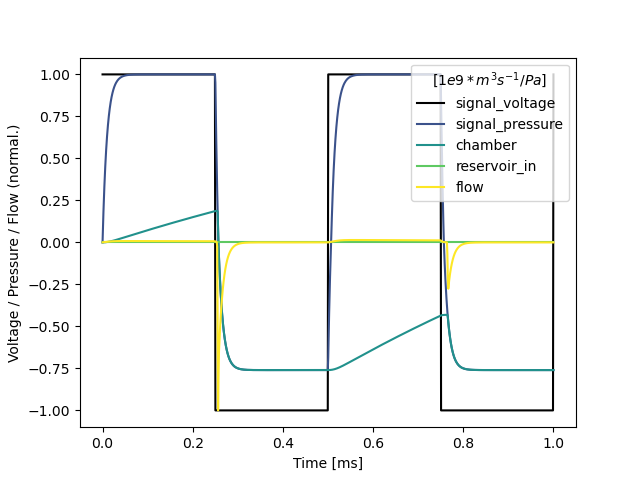
\includegraphics[width=\textwidth, valign=t]{bilder/leakage/leakage_in_branch_singleweep.png}
	\end{subfigure}
	\begin{subfigure}[H]{0.48\textwidth}
		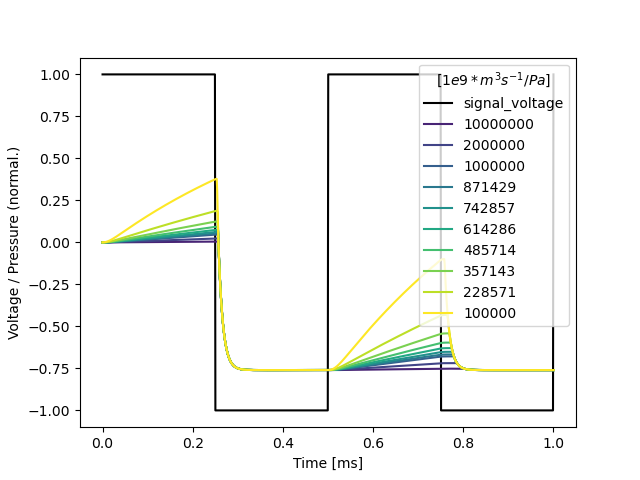
\includegraphics[width=\textwidth, valign=t]{bilder/leakage/leakage_in_branch_multiweep.png}
	\end{subfigure}
    \caption{a) Volumenstrom- und Druckverläufe eines nicht verschließenden Klappenventils, b) Druckverläufe für variierte Verschluss-Widerstandswerte}
    \label{fig:leckagedruck}
\end{figure}

\begin{figure}[H]
	\centering
	\begin{subfigure}[H]{0.48\textwidth}
		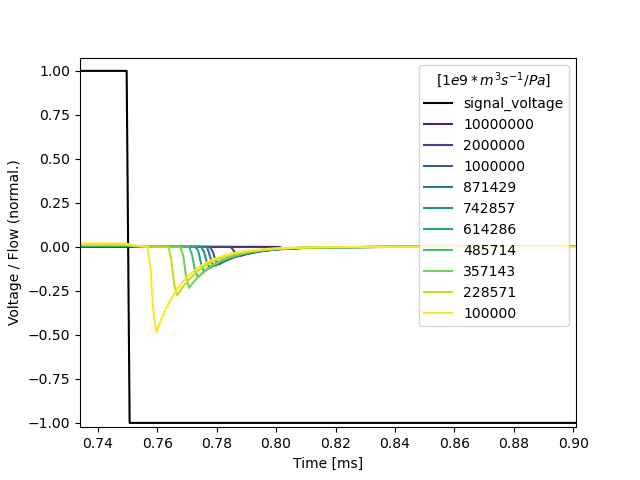
\includegraphics[width=\textwidth, valign=t]{bilder/leakage/leakage_in_branch_multiweep_flow.png}
	\end{subfigure}
    \caption{Pumpstromverläufe für variierte Verschluss-Widerstandswerte während des zweiten Saughubs}
    \label{fig:leckagestrom}
\end{figure}

\subsection{Leitungen}

Abhängig vom Einsatzbereich und Einbauverhältnis können variierende Leitungslängen zwischen Pumpe und den jeweiligen Reservoirs auftreten. Um die eintretenden Effekte zu visualisieren sind hier relativ hohe Leitungslängen angenommen worden. Jedoch ist ein qualitativ ähnliches Verhalten für geringere Längen-Variationen zu erwarten. Abbildung \ref{fig:zuleitungen} zeigt die Ausgangssituation und den verzögerten Druckaufbau für erhöhte Zuleitungs-Längen für die Saughub-Phasen. Wie in Abschnitt \ref{subsec:reservoirsection} beschrieben steht der Strömungswiderstand der Leitung in linearen Zusammenhang mit ihrer Länge (Gleichung \ref{eq:leckagestrom}). Der verzögerte Druckaufbau (wie er analog auch in Abbildung \ref{fig:sweepleitungen} zu beobachten ist) führt zu einem abgesenkten Volumenstrom, der aber länger anhält (siehe Abbildung \ref{fig:sweepströme}). Das von der Pumpe beförderte Volumen ergibt sich aus der Fläche unter der jeweiligen Kurve. Ein den Volumenstrom beschränkender Faktor wäre dann eine erhöhte Frequenz, die einen verzögerten Druckaufbau bis zum Endwert nicht mehr zulässt.

\begin{figure}[H]
	\centering
	\begin{subfigure}[H]{0.48\textwidth}
		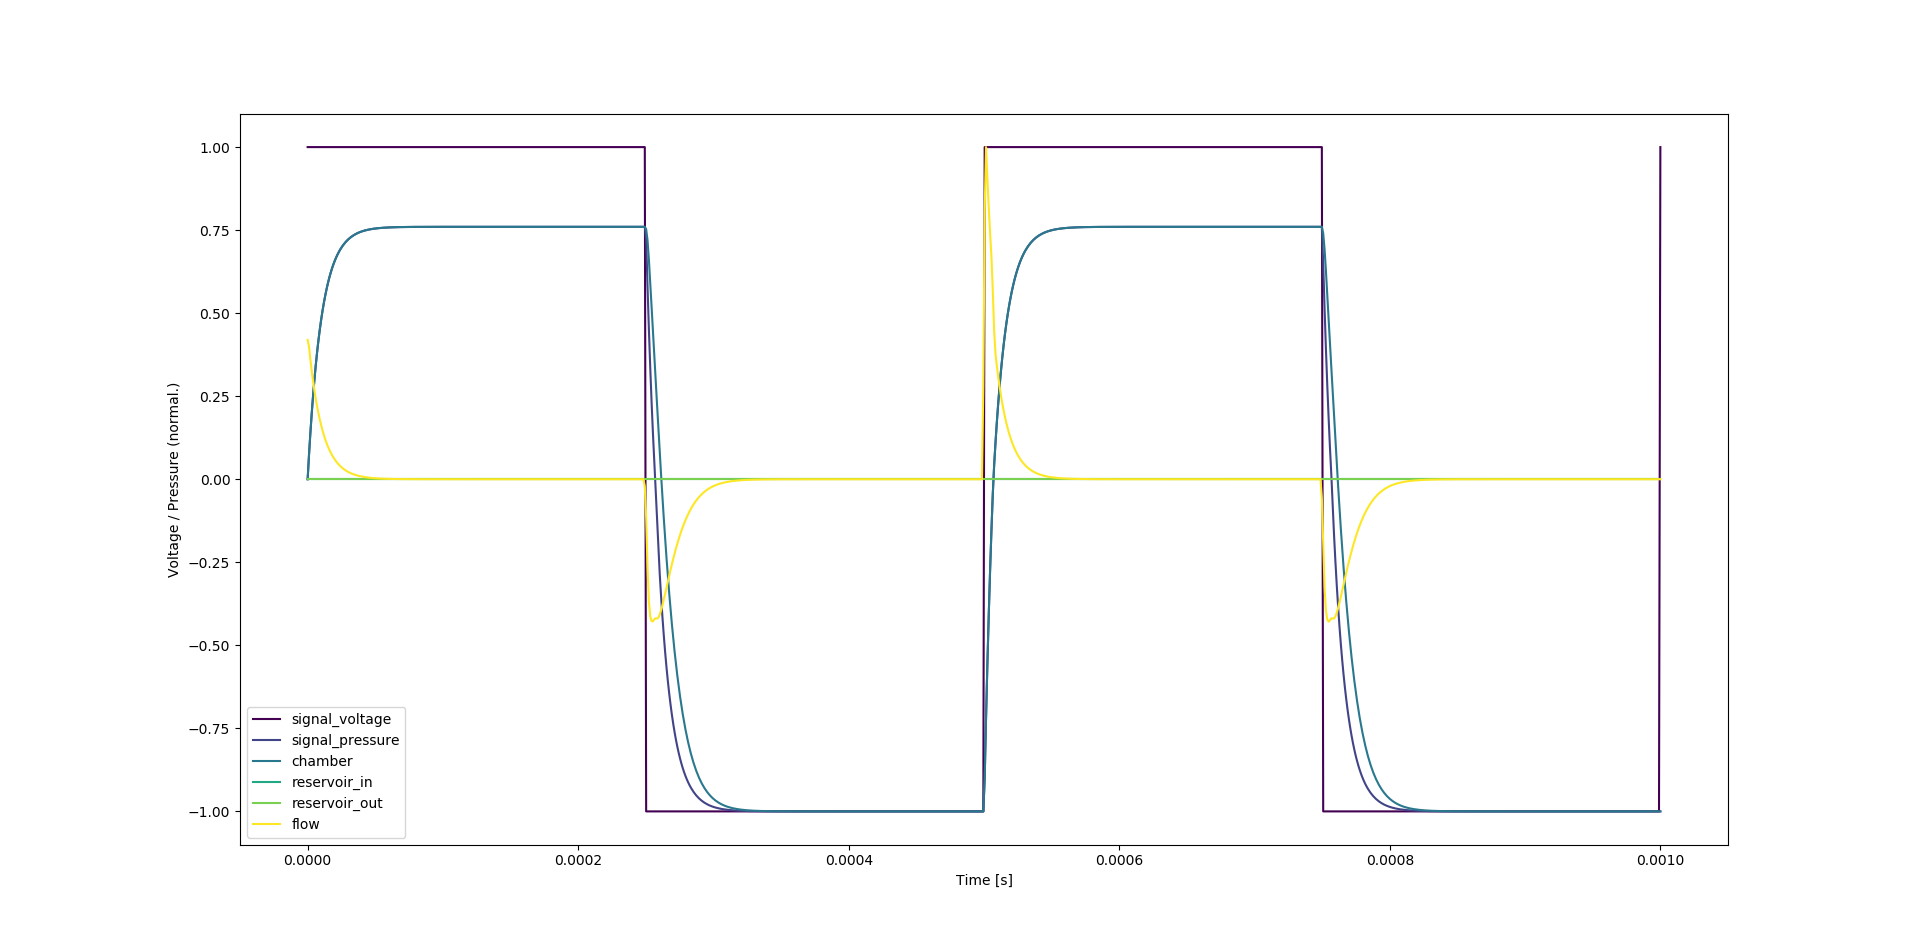
\includegraphics[width=\textwidth, valign=t]{bilder/tubelength/tl_in_branch_singlesweep.png}
	\end{subfigure}
	\begin{subfigure}[H]{0.48\textwidth}
		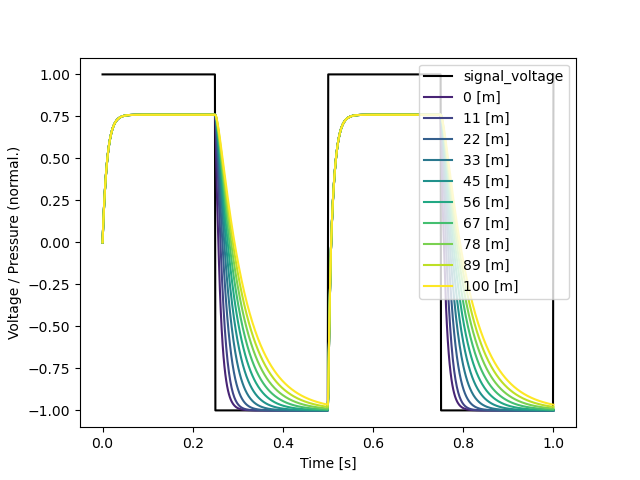
\includegraphics[width=\textwidth, valign=t]{bilder/tubelength/tl_in_branch_multisweep.png}
	\end{subfigure}
    \caption{a) Volumenstrom- und Druckverläufe für geringe Zuleitungs-Länge b) Variation der Zuleitungs-Länge}
    \label{fig:zuleitungen}
\end{figure}

\begin{figure}[H]
	\centering
	\begin{subfigure}[H]{0.48\textwidth}
		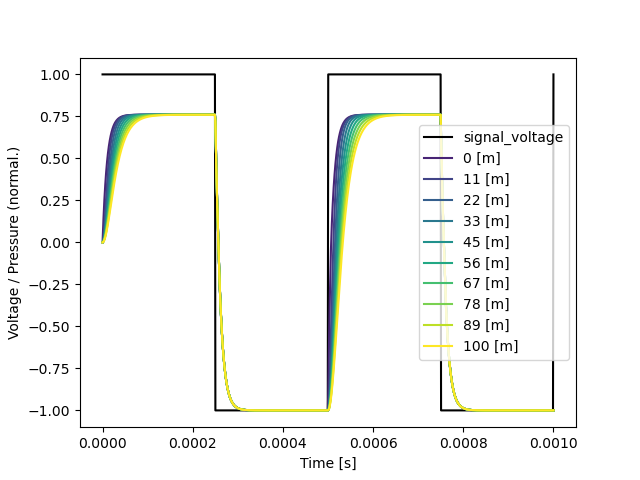
\includegraphics[width=\textwidth, valign=t]{bilder/tubelength/tl_out_branch_multisweep.png}
	\end{subfigure}
	\begin{subfigure}[H]{0.48\textwidth}
		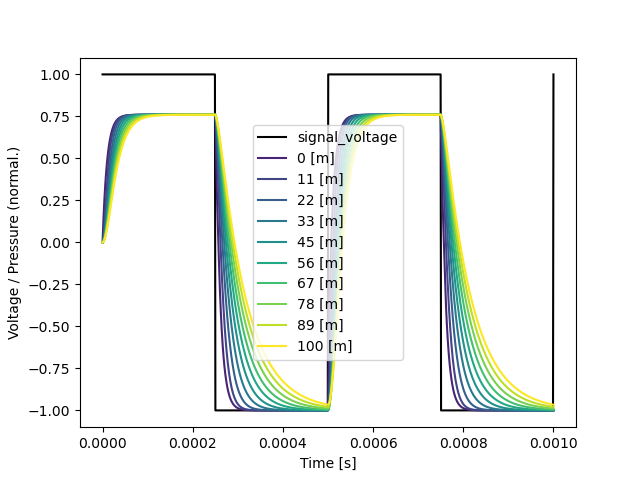
\includegraphics[width=\textwidth, valign=t]{bilder/tubelength/tl_both_branch_multisweep.png}
	\end{subfigure}
    \caption{a) Variation der Ausleitungs-Länge b) Variation beider Leitungs-Längen}
    \label{fig:sweepleitungen}
\end{figure}

\begin{figure}[H]
	\centering
	\begin{subfigure}[H]{0.48\textwidth}
		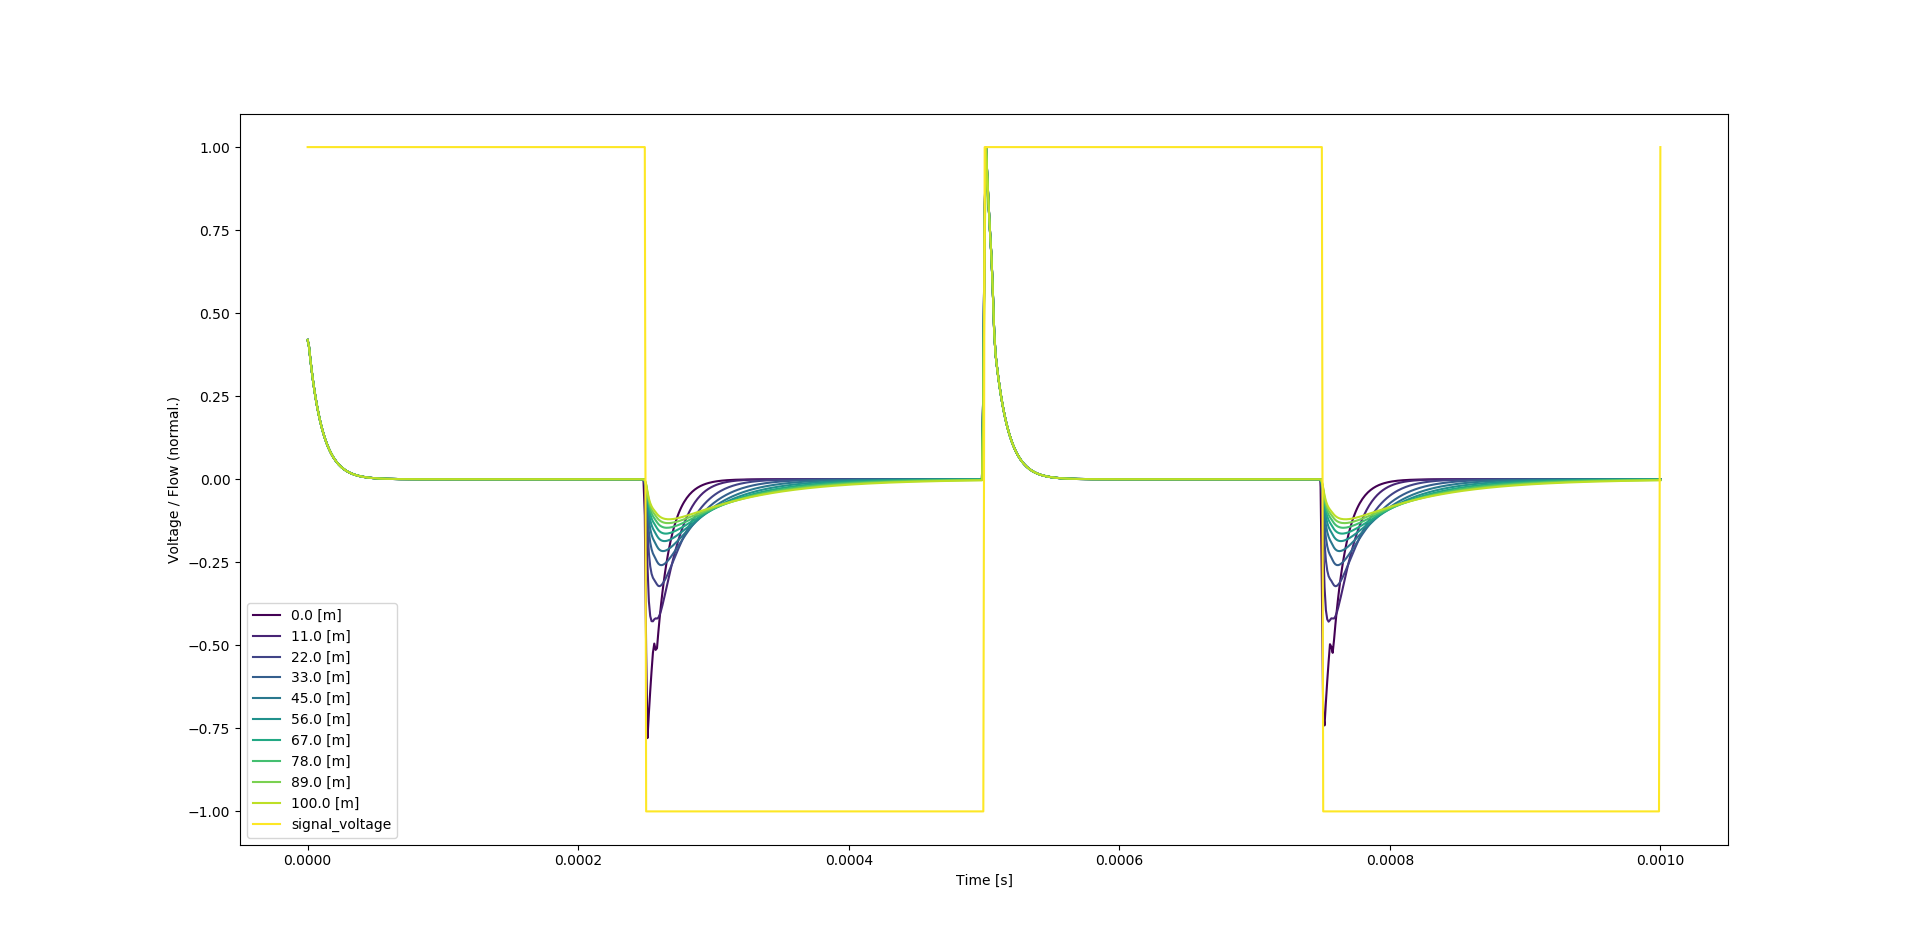
\includegraphics[width=\textwidth, valign=t]{bilder/tubelength/tl_in_branch_multisweep_flow.png}
	\end{subfigure}
	\begin{subfigure}[H]{0.48\textwidth}
	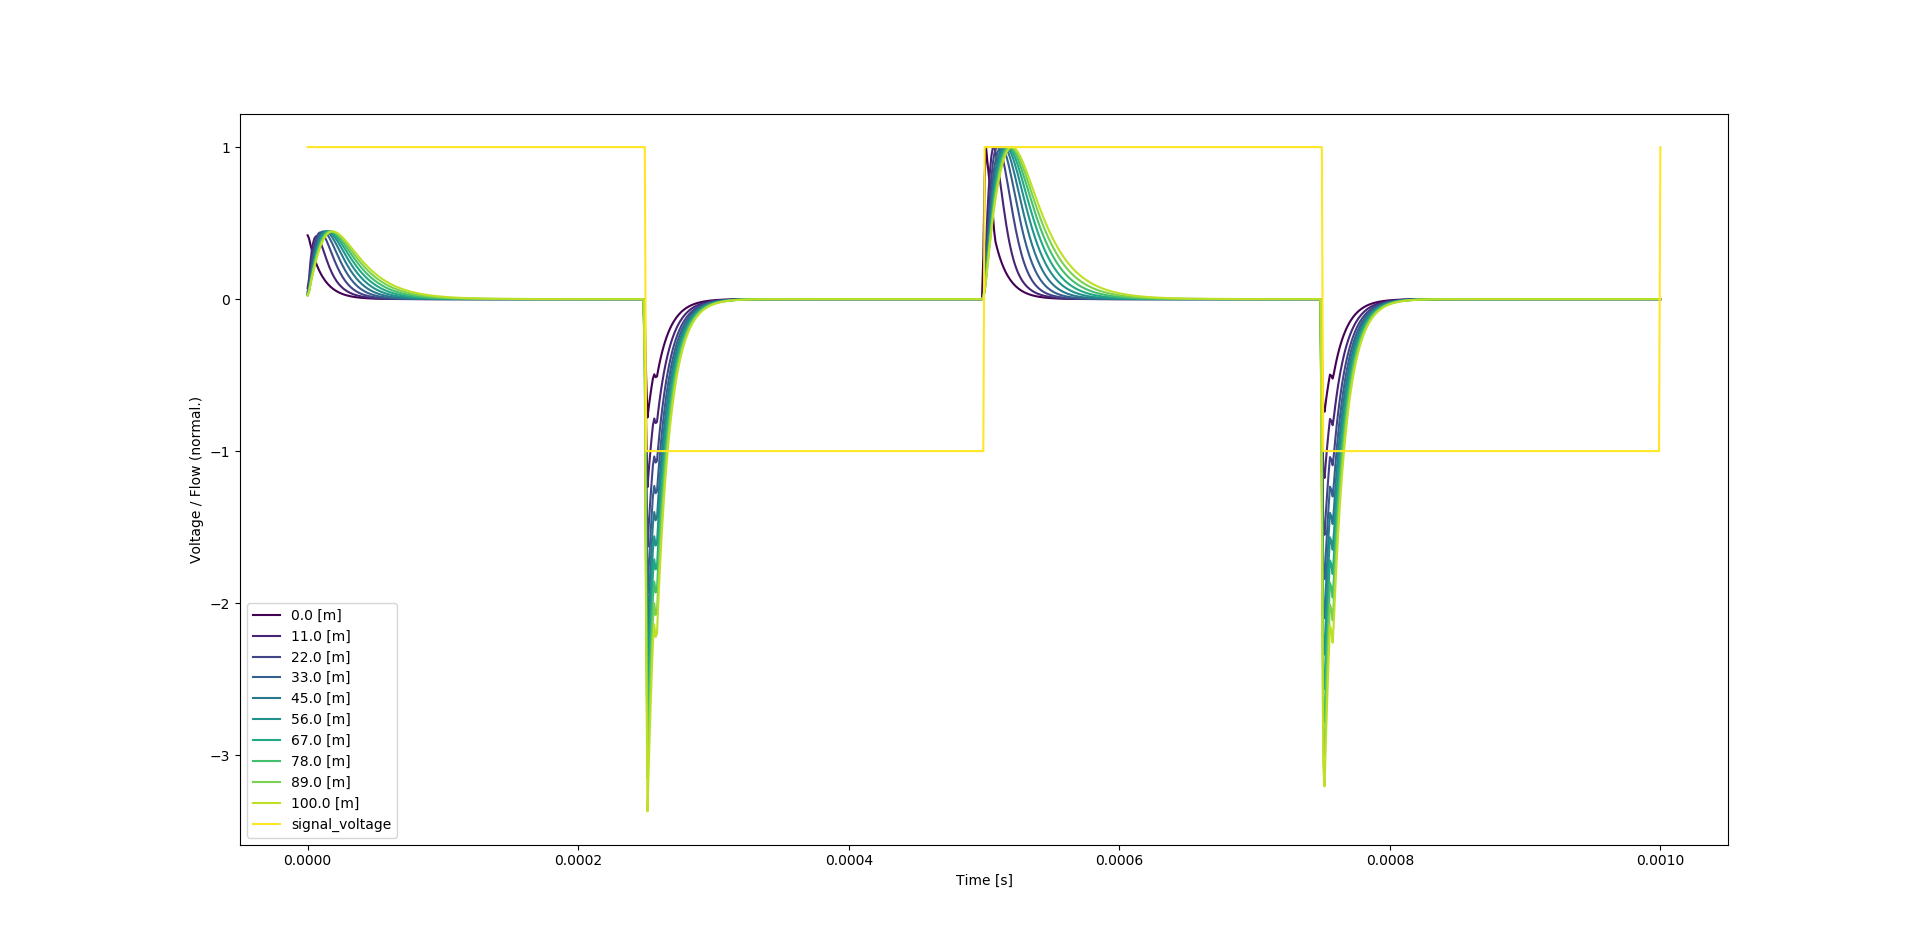
\includegraphics[width=\textwidth, valign=t]{bilder/tubelength/tl_out_branch_multisweep_flow.png}
	\end{subfigure}
	\begin{subfigure}[H]{0.48\textwidth}
		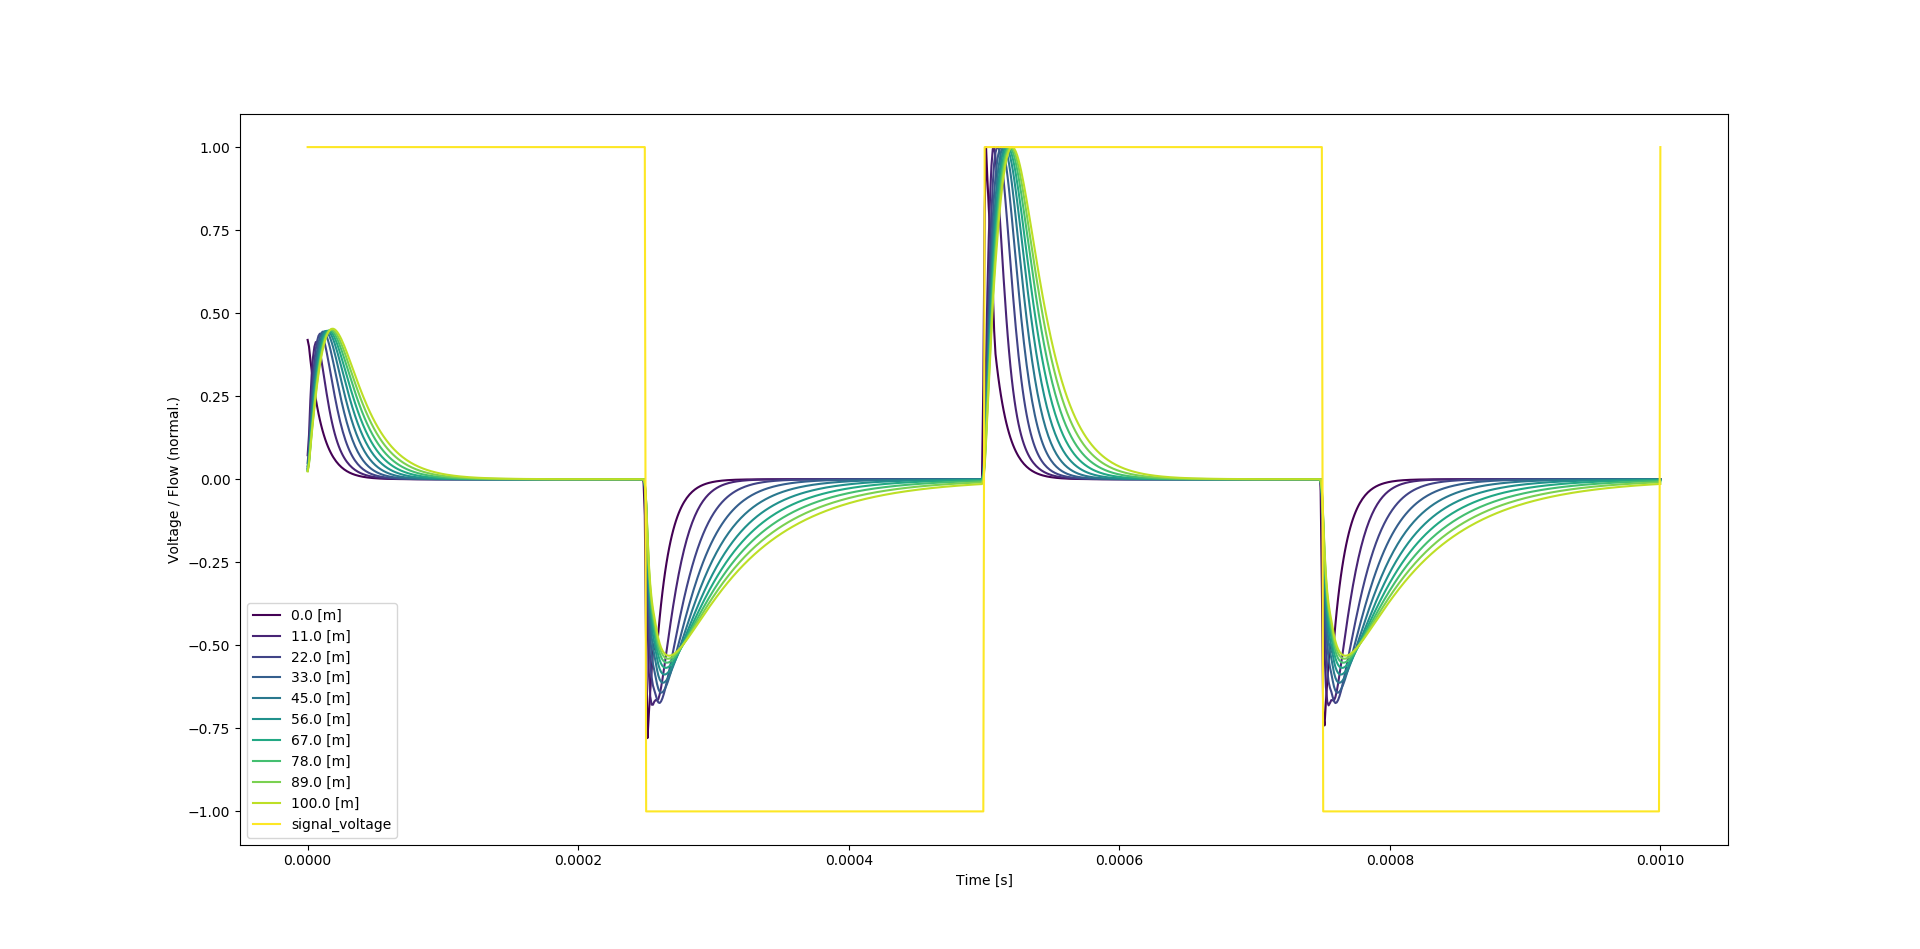
\includegraphics[width=\textwidth, valign=t]{bilder/tubelength/tl_both_branch_multisweep_flow.png}
	\end{subfigure}
    \caption{Volumenstromverläufe für Längenvariation von a) Zuleitungen b) Ausleitungen c) beider Leitungen}
    \label{fig:sweepströme}
\end{figure}

\subsection{Gegendruck}

Ansteuerung und Auslenkung vertauscht?

Zur Bestimmung des maximalen Druckes, welcher in der Pumpkammer aufgebaut wird, ist eine Simulation bei veränderlichem Druck der Reservoire durchzuführen. Für die folgende Simulation wird die Pumpe mit einem Rechtecksignal bei einer Frequenz von 2 kHz angesteuert. In Abbildung \ref{fig:gegendruck_all} a) ist der Druck in der Pumpkammer zu sehen. Der externe Druck der Reservoire beträgt kPa. In Abbildung \ref{fig:gegendruck_all} b) ist die Ansteuerung identisch, nur sind in diesem Fall die externen Drücke höher. Der Druck am Einlassventil ist höher als der Druck in der Pumpkammer während einem Saughub wodurch kein effektiver Druck entsteht, welcher zu einem Stromfluss führt. Im Fall des Auslassventiles reicht kann die Pumpkammer gerade noch so gegen den extern angelegten Druckarbeiten was in der geringen Amplitude währen dem Druckhub zu erkennen ist.

\begin{figure}[H]
    \centering
    \begin{subfigure}[H]{0.48\textwidth}
        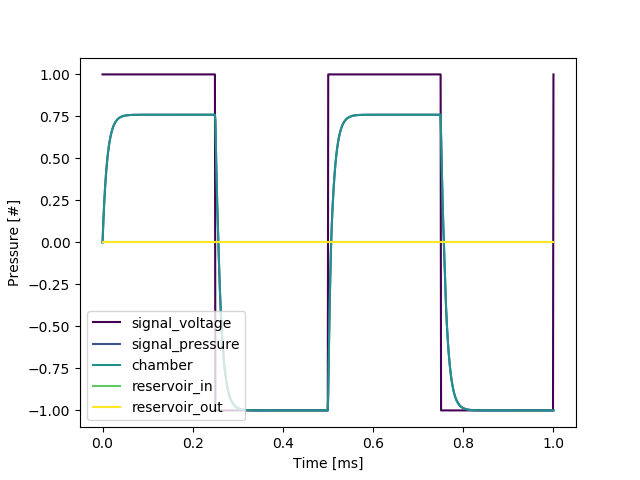
\includegraphics[width=\textwidth, valign=t]{bilder/backpressure/backpressure_free.png}
    \end{subfigure}
    \begin{subfigure}[H]{0.48\textwidth}
        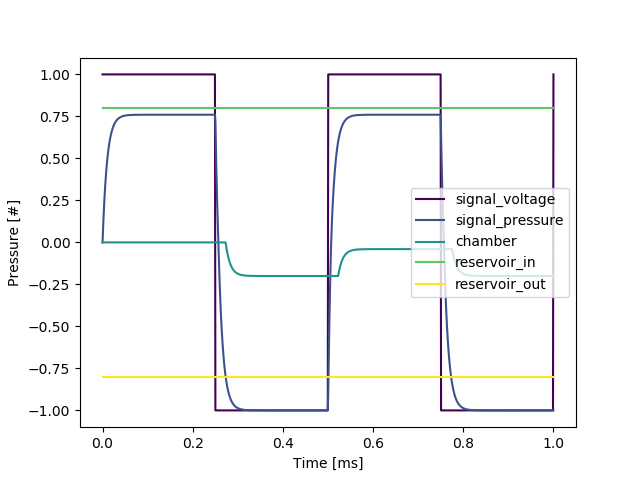
\includegraphics[width=\textwidth, valign=t]{bilder/backpressure/backpressure_example.png}
    \end{subfigure}
    \begin{subfigure}[H]{0.48\textwidth}
        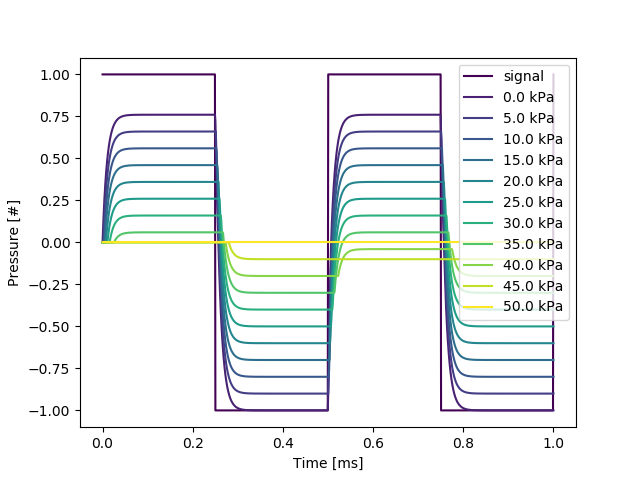
\includegraphics[width=\textwidth, valign=t]{bilder/backpressure/backpressure_at_pr_in_and_pr_out.png}
    \end{subfigure}
    \begin{subfigure}[H]{0.48\textwidth}
        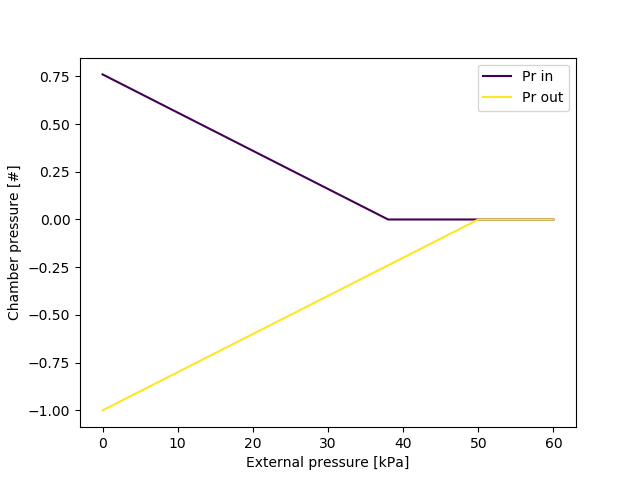
\includegraphics[width=\textwidth, valign=t]{bilder/backpressure/backpressure_result.png}
    \end{subfigure}
    \caption{a) Ohne externen Gegendruck b) Mit externem Gegendruck an Ein- und Auslass. c) Variation der Gegendrücke an Ein- und Auslassventil. d) Maximaler Gegendruck bei dem die Amplitude an Ein- und Auslassventil auf null abfällt.}
    \label{fig:gegendruck_all}
\end{figure}

Zur Bestimmung des maximalen Gegendruckes werden nun die Drücke an den beiden Reservoirs variiert. Dazu wird am Einlassventil ein Überdruck und am Auslassventil ein Unterdruck angelegt. Die Auswirkungen auf das Signal des Druckes in der Pumpkammer ist Abbildung \ref{fig:gegendruck_all} c) zu entnehmen. Da hier jedoch nicht der genaue Druck bestimmt werden kann bei dem die Pumpe aufhört zu pumpen wird die Simulation mit einer geringen Schrittweite der Gegendrücke durchgeführt. Das Ergebnis dieser Simulation ist in Abbildung \ref{fig:gegendruck_all} d) zu sehen. Der maximale Gegendruck für das Einlassventil beträgt demnach 38 kPa und für das Auslassventil 50 kPa. Da die Ventile ideal sind entspricht der maximale Gegendruck genau der maximalen Amplitude des Druckes in der Pumpkammer. Bei realen Ventilen, welche zum Öffnen einen Über- bzw. Unterdruck benötigen würde die Pumpe schon bei geringeren externen Drücken zum erliegen kommen.

\subsection{Grenzfrequenz}

Um die maximale Betriebsfrequenz der Pumpe zu bestimmen wird eine Variation der Antriebsfrequenz simuliert. Da die Pumpe eine Trägheit besitzt welche durch ein RC-Glied beschrieben wird, kann die Pumpe nicht mit beliebig hohen Frequenzen betrieben werden. Das Spannungssignal in der Pumpe ist in Abbildung \ref{fig:frequency_all} a) zu sehen. Die Antriebsfrequenz des Aktors beträgt 1 kHz. Es ist gut zu erkennen das die Anstiegszeit des Pumpkammerdruckes ausreicht um die maximale Druckamplitude in der Pumpkammer aufzubauen. In Abbildung \ref{fig:frequency_all} b) ist das Verhalten bei hohen Frequenzen zu sehen, die Frequenz beträgt hier etwas mehr als 11 kHz. Bei dieser hohen Frequenz ist die Auslenkung des Aktors zu träge und das Signal der Pumpkammer kann dem Eingangssignal nicht mehr folgen, was zu einer Minderung der Pumpleistung führt, die Abhängigkeit der Amplitude von der Frequenz ist über den Frequenzbereich von 2 kHz bis zu 200 kHz ist in Abbildung \ref{fig:frequency_all} c) zu sehen.
 
\begin{figure}[H]
    \centering
    \begin{subfigure}[H]{0.48\textwidth}
        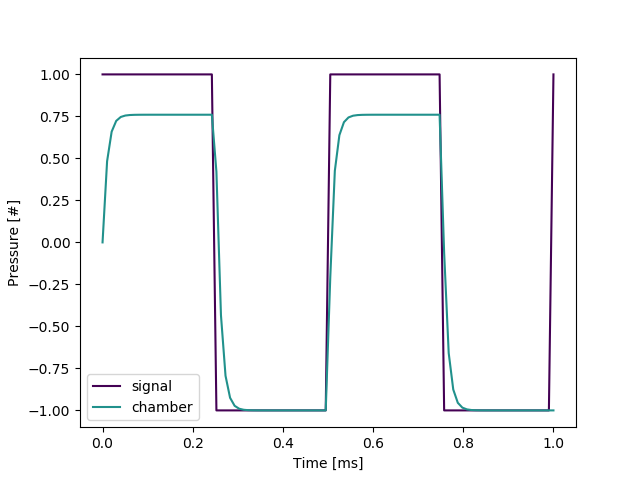
\includegraphics[width=\textwidth, valign=t]{bilder/frequency/frequency_default_2kHz.png}
    \end{subfigure}
    \begin{subfigure}[H]{0.48\textwidth}
        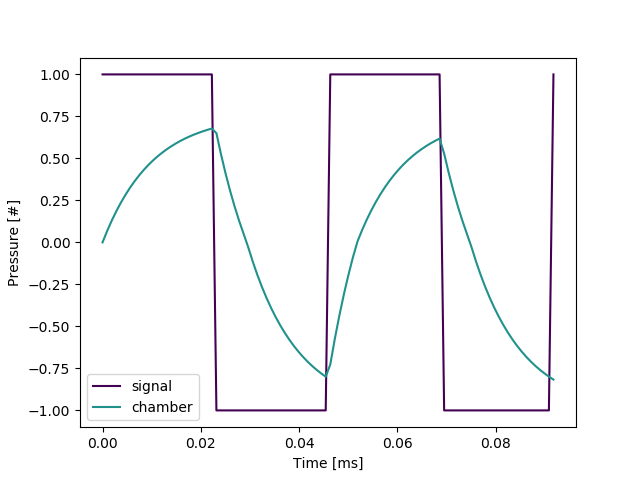
\includegraphics[width=\textwidth, valign=t]{bilder/frequency/frequency_to_fast_21_8 khz.png}
    \end{subfigure}
    \begin{subfigure}[H]{0.48\textwidth}
        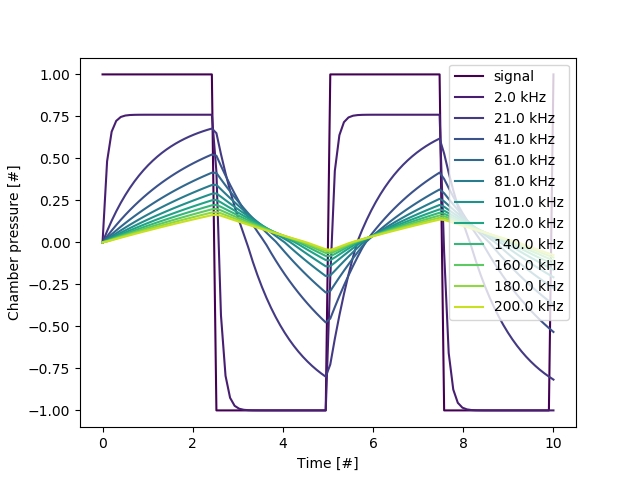
\includegraphics[width=\textwidth, valign=t]{bilder/frequency/frequency_sweep.png}
    \end{subfigure}
    \begin{subfigure}[H]{0.48\textwidth}
        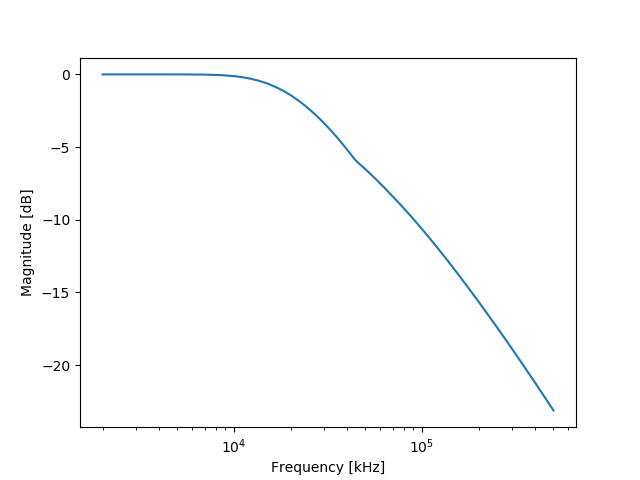
\includegraphics[width=\textwidth, valign=t]{bilder/frequency/bode_diagram.png}
    \end{subfigure}
    \caption{a) Ansteuerung der Pumpe bei 1 kHz. b) Ansteuerung der Pumpe bei 11 kHz, der Aktor kann dem Eingangssignal nicht mehr folgen. c) Variation der Antriebsfrequenz zwischen 2 kHz und 200 kHz. d) Darstellung der Frequenzabhängigkeit der Amplitude im Bode-Diagramm.}
    \label{fig:frequency_all}
\end{figure}

Für die Darstellung des frequenzabhängigen Verhaltens der Membranpumpe werden Frequenzen bis zu 500 kHz simuliert. Die dabei resultierende Amplitude wird in einem Bode-Diagramm über die Frequenz aufgetragen. Nun kann die Grenzfrequenz bestimmt werden, welche bei -3 dB liegt. Die Grenzfrequenz beträgt demnach 28,3 kHz.

\section{Fazit}

Im Rahmen dieser Simulationsstudie konnte gezeigt werden, das mit einem relativ einfachen Simulationsmodel in erster Ordnung weitreichende Untersuchungen bezüglich der einzelnen Teilkomponenten sowie des Gesamtsystems durchgeführt werden können. Mit der Simulation der Zuleitungen im Einzelstrang konnte eine Abschätzung der maximalen Rohrlänge gemacht werden. Ebenso ist mittels dem Einzelstrang-Modell ein Messprinzip zur Untersuchung der Dichtheit der Klappenventile definiert worden. Mittels der Modellierung des Gesamtsystems wurde ein Messprinzip definiert um den maximalen Druck in der Pumpkammer zu bestimmen. Mit der finalen Simulation der Betriebsfrequenz der Pumpe konnte die Grenzfrequenz des Systems abgeschätzt werden. Im Folgenden Abschnitt wird die Erweiterung des in dieser Arbeit erstellten Modells behandelt.

\section{Ausblick}

Das Systemmodell kann hinsichtlich der einzelnen Komponenten nahezu beliebig komplex erweitert werden. Um einen Einblick zu erlangen, welche Konsequenzen ein höherer Detailierungsgrad nach sich zieht, wird die Beschreibung der Ventile, der Rohrleitungen und der Pumpkammer erweitert. Die geometrische Gestaltung der Pumpkammer führt zu Strömungswiderständen, welche in einem Widerstand $R_C$ zusammengefasst werden können. Das Ventil besitzt durch die zugrundeliegende Geometrie auch kapazitive Eigenschaften, verursacht durch elastische Verformungen des Bauteils. Dieser Effekt wird im folgenden Modell durch parallele Kondensatoren ($C_{V_{in}}$ und $C_{V_{out}}$) berücksichtigt. Zusätzlich kann der Fluid-inherente Widerstand gegen Beschleunigungen innerhalb von Rohrleitungen durch eine Induktivität ($L_{V_{in}}$ und $L_{V_{out}}$) beschrieben werden. Dabei gilt folgende elektro-fluidische Analogie:


\begin{equation}
	L_{fluid} = \frac{P}{\ddot{V}} \:\:\widehat{=}\:\: L_{elek.} = \frac{U}{dI/dt}
\end{equation}

\begin{equation}
	I_{C} = I_{in} + I_{out}
\end{equation}

\begin{figure}[H]
	\includesvg[scale = 0.6]{bilder/circuits/second_order_circuit}
	\caption{Erweitertes Pumpenmodell in Ersatzschaltbild-Darstellung}
	\label{outlookcircuit}
\end{figure}

Eine Herleitung der Differentialgleichung nach den Kirchhoffschen Regeln führt für dargestelltes System (siehe Abbildung \ref{outlookcircuit}) zu folgendem Zusammenhang nach Trennung der Variablen:

\begin{equation}
	\begin{split}
		&+ \left[\left(1+\frac{R_{T_{out}}}{R_{V_{out}}}\right)C_{V_{in}}L_{T_{in}}C_{C}\right]\bm{\frac{d\textsuperscript{3}U_{C}}{dt\textsuperscript{3}}} \\
		&+ \left[\left(1+\frac{R_{T_{out}}}{R_{V_{out}}}\right)C_{V_{in}}R_{C}C_{C} + \left(1+\frac{R_{T_{in}}}{R_{V_{in}}}\right)C_{V_{out}}R_{C}C_{C}\right]\bm{\frac{d\textsuperscript{2}U_{C}}{dt\textsuperscript{2}}} \\
		&+ \biggl[\left(1+\frac{R_{T_{in}}}{R_{V_{in}}}\right)\left(1+\frac{R_{T_{out}}}{R_{V_{out}}}\right)C_{C} + \left(1+\frac{R_{T_{out}}}{R_{V_{out}}}\right)\left(\frac{R_{C}C_{C}}{R_{V_{in}}}+C_{V_{in}}\right) + \\
		& \left(1+\frac{R_{T_{in}}}{R_{V_{in}}}\right)\left(\frac{R_{C}C_{C}}{R_{V_{out}}}+C_{V_{out}}\right)\biggr] \bm{\frac{dU_{C}}{dt}}  \\
		&+ \left[\left(1+\frac{R_{T_{out}}}{R_{V_{out}}}\right)\frac{1}{R_{V_{in}}} + \left(1+\frac{R_{T_{in}}}{R_{V_{in}}}\right)\frac{1}{R_{V_{out}}}\right]\bm{U_{C}} \\
		&= \left[\left(1+\frac{R_{T_{out}}}{R_{V_{out}}}\right)C_{V_{in}}L_{T_{in}} - \left(1+\frac{R_{T_{in}}}{R_{V_{in}}}\right)C_{V_{out}}L_{T_{out}}\right]\bm{\frac{d\textsuperscript{2}I_{out}}{dt\textsuperscript{2}}} \\
		&+ \biggl[\left(1+\frac{R_{T_{out}}}{R_{V_{out}}}\right)\left(\frac{L_{T_{in}}}{R_{V_{in}}}+C_{V_{in}}R_{V_{in}}\right) - \left(1+\frac{R_{T_{in}}}{R_{V_{in}}}\right)\left(\frac{L_{T_{out}}}{R_{V_{out}}}+C_{V_{out}}R_{V_{out}}\right)\biggr]\bm{\frac{dI_{out}}{dt}} \\
		&+ \left(1+\frac{R_{T_{out}}}{R_{V_{out}}}\right)C_{V_{in}}\bm{\frac{d(U_{Signal}(t) - U_{in})}{dt}} + \left(1+\frac{R_{T_{out}}}{R_{V_{out}}}\right)\frac{1}{R_{T_{in}}}\bm{(U_{Signal}(t) - U_{in})} \\
		&+ \left(1+\frac{R_{T_{in}}}{R_{V_{in}}}\right)C_{V_{out}}\bm{\frac{d(U_{Signal}(t) - U_{out})}{dt}} + \left(1+\frac{R_{T_{in}}}{R_{V_{in}}}\right)\frac{1}{R_{T_{out}}}\bm{(U_{Signal}(t) - U_{out})}
	\end{split}
\end{equation}

\pagebreak
Es handelt sich dabei um eine lineare, inhomogene DGL dritter Ordnung, die sich evtl. durch weiteres Umformen von den $I_{out}$ Termen entledigen kann. Um sich dessen zu vergewissern würden sich symbolische Mathematik-Solver wie Maple oder Mathematica anbieten. Eine entsprechende Implementierung wurde nicht vorgenommen und würde die Festlegung zusätzlicher Randbedingungen erfordern.

\newpage

\bibliography{sim_axelsson}
\bibliographystyle{plain}

\end{document}
